\documentclass{standalone}
\usepackage{tikz}
\usetikzlibrary{patterns, positioning}
\usepackage[sfdefault]{ClearSans} %% option 'sfdefault' activates Clear Sans as the default text font
\usepackage[T1]{fontenc}

\begin{document}
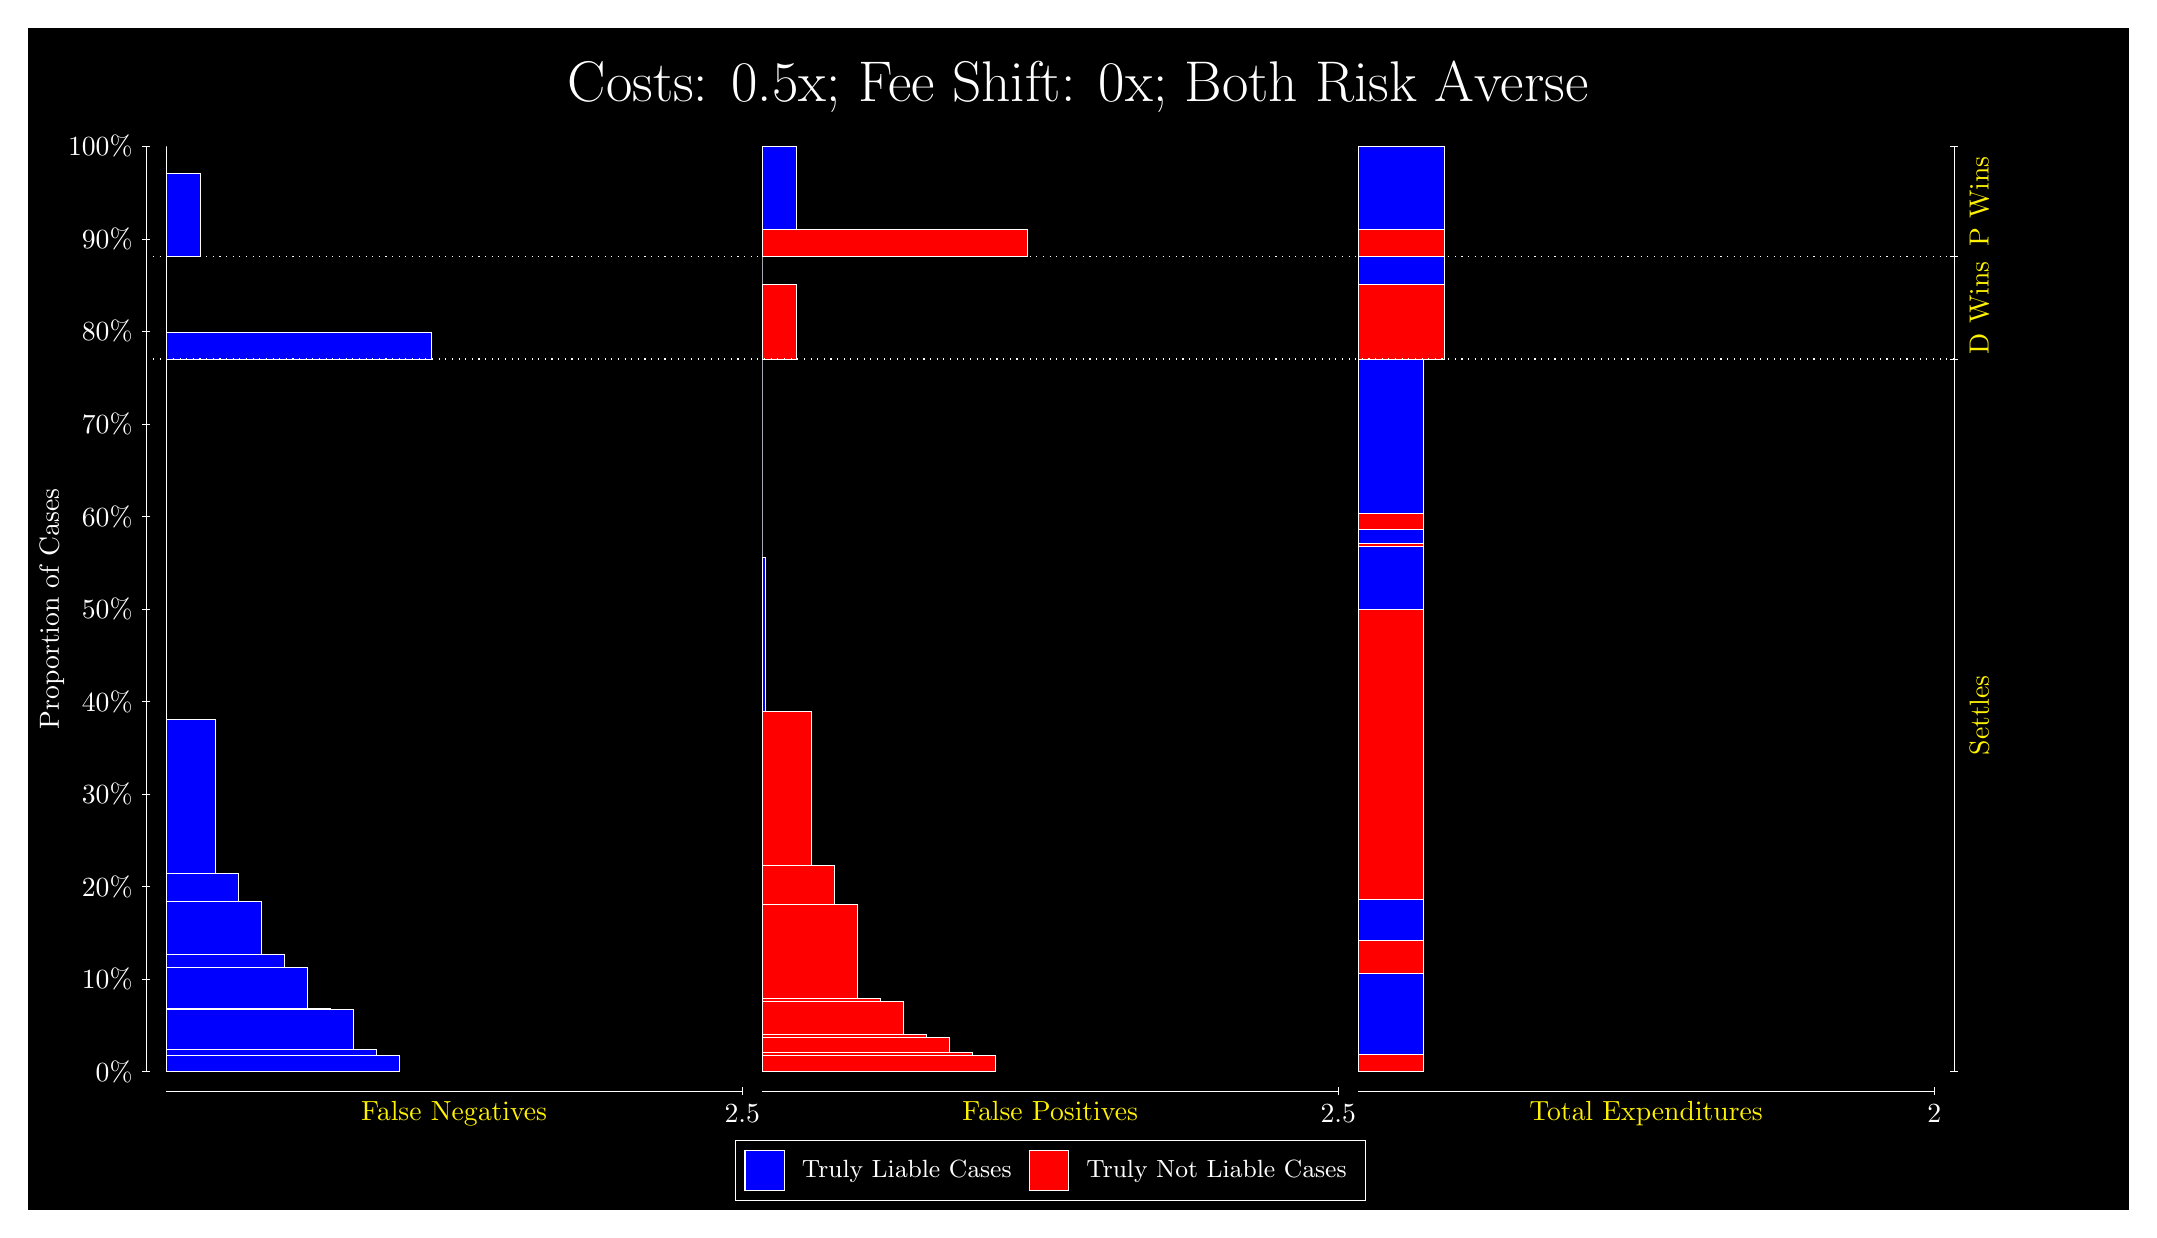
\begin{tikzpicture}
\draw[fill=black] (0,0) rectangle (26.667,15);
\draw[text=white] (0,13.5) rectangle (26.667,15) node[midway] {\huge Costs: 0.5x; Fee Shift: 0x; Both Risk Averse};
\draw[white, very thin] (1.5,1.75) -- (1.5,13.5);
\node[rotate=90, text=white, anchor=center] at (0.3, 7.625) {Proportion of Cases};
\draw[white, very thin] (1.45,1.75) -- (1.55,1.75);
\node[text=white, anchor=east] at (1.45, 1.75) {0\%};
\draw[white, very thin] (1.45,2.925) -- (1.55,2.925);
\node[text=white, anchor=east] at (1.45, 2.925) {10\%};
\draw[white, very thin] (1.45,4.1) -- (1.55,4.1);
\node[text=white, anchor=east] at (1.45, 4.1) {20\%};
\draw[white, very thin] (1.45,5.275) -- (1.55,5.275);
\node[text=white, anchor=east] at (1.45, 5.275) {30\%};
\draw[white, very thin] (1.45,6.45) -- (1.55,6.45);
\node[text=white, anchor=east] at (1.45, 6.45) {40\%};
\draw[white, very thin] (1.45,7.625) -- (1.55,7.625);
\node[text=white, anchor=east] at (1.45, 7.625) {50\%};
\draw[white, very thin] (1.45,8.8) -- (1.55,8.8);
\node[text=white, anchor=east] at (1.45, 8.8) {60\%};
\draw[white, very thin] (1.45,9.975) -- (1.55,9.975);
\node[text=white, anchor=east] at (1.45, 9.975) {70\%};
\draw[white, very thin] (1.45,11.15) -- (1.55,11.15);
\node[text=white, anchor=east] at (1.45, 11.15) {80\%};
\draw[white, very thin] (1.45,12.325) -- (1.55,12.325);
\node[text=white, anchor=east] at (1.45, 12.325) {90\%};
\draw[white, very thin] (1.45,13.5) -- (1.55,13.5);
\node[text=white, anchor=east] at (1.45, 13.5) {100\%};

\draw[white, very thin] (24.457,1.75) -- (24.457,13.5);
\draw[white, very thin] (24.407,1.75) -- (24.507,1.75);
\node[anchor=west] at (24.407, 1.75) {};
\draw[white, very thin] (24.407,10.799) -- (24.507,10.799);
\node[anchor=west] at (24.407, 10.799) {};
\draw[white, very thin] (24.407,12.098) -- (24.507,12.098);
\node[anchor=west] at (24.407, 12.098) {};
\draw[white, very thin] (24.407,13.5) -- (24.507,13.5);
\node[anchor=west] at (24.407, 13.5) {};

\draw[white, very thin, fill=blue] (1.75,1.75) rectangle (4.7141,1.96);
\draw[white, very thin, fill=blue] (1.75,1.96) rectangle (4.4214,2.0268);
\draw[white, very thin, fill=blue] (1.75,2.0268) rectangle (4.1286,2.5414);
\draw[white, very thin, fill=blue] (1.75,2.5414) rectangle (3.8359,2.5548);
\draw[white, very thin, fill=blue] (1.75,2.5548) rectangle (3.5431,3.079);
\draw[white, very thin, fill=blue] (1.75,3.079) rectangle (3.2504,3.2448);
\draw[white, very thin, fill=blue] (1.75,3.2448) rectangle (2.9576,3.9111);
\draw[white, very thin, fill=blue] (1.75,3.9111) rectangle (2.6649,4.2642);
\draw[white, very thin, fill=blue] (1.75,4.2642) rectangle (2.3721,6.2233);
\draw[white, very thin, fill=red] (1.75,6.2233) rectangle (1.75,10.799);
\draw[white, very thin, fill=blue] (1.75,10.799) rectangle (5.1167,11.144);
\draw[white, very thin, fill=red] (1.75,11.144) rectangle (1.75,12.098);
\draw[white, very thin, fill=blue] (1.75,12.098) rectangle (2.1891,13.155);
\draw[white, very thin, fill=red] (1.75,13.155) rectangle (1.75,13.5);
\draw[white, very thin, fill=red] (9.3189,1.75) rectangle (12.283,1.96);
\draw[white, very thin, fill=red] (9.3189,1.96) rectangle (11.99,1.9982);
\draw[white, very thin, fill=red] (9.3189,1.9982) rectangle (11.697,2.1836);
\draw[white, very thin, fill=red] (9.3189,2.1836) rectangle (11.405,2.2256);
\draw[white, very thin, fill=red] (9.3189,2.2256) rectangle (11.112,2.6472);
\draw[white, very thin, fill=red] (9.3189,2.6472) rectangle (10.819,2.6768);
\draw[white, very thin, fill=red] (9.3189,2.6768) rectangle (10.526,3.8776);
\draw[white, very thin, fill=red] (9.3189,3.8776) rectangle (10.234,4.3669);
\draw[white, very thin, fill=red] (9.3189,4.3669) rectangle (9.941,6.3261);
\draw[white, very thin, fill=blue] (9.3189,6.3261) rectangle (9.3555,8.2852);
\draw[white, very thin, fill=blue] (9.3189,8.2852) rectangle (9.3189,10.799);
\draw[white, very thin, fill=red] (9.3189,10.799) rectangle (9.758,11.753);
\draw[white, very thin, fill=blue] (9.3189,11.753) rectangle (9.3189,12.098);
\draw[white, very thin, fill=red] (9.3189,12.098) rectangle (12.686,12.443);
\draw[white, very thin, fill=blue] (9.3189,12.443) rectangle (9.758,13.5);
\draw[white, very thin, fill=red] (16.888,1.75) rectangle (17.711,1.9736);
\draw[white, very thin, fill=blue] (16.888,1.9736) rectangle (17.711,2.993);
\draw[white, very thin, fill=red] (16.888,2.993) rectangle (17.711,3.4146);
\draw[white, very thin, fill=blue] (16.888,3.4146) rectangle (17.711,3.9388);
\draw[white, very thin, fill=red] (16.888,3.9388) rectangle (17.711,7.6177);
\draw[white, very thin, fill=blue] (16.888,7.6177) rectangle (17.711,8.4225);
\draw[white, very thin, fill=red] (16.888,8.4225) rectangle (17.711,8.4645);
\draw[white, very thin, fill=blue] (16.888,8.4645) rectangle (17.711,8.6303);
\draw[white, very thin, fill=red] (16.888,8.6303) rectangle (17.711,8.8403);
\draw[white, very thin, fill=blue] (16.888,8.8403) rectangle (17.711,10.799);
\draw[white, very thin, fill=red] (16.888,10.799) rectangle (17.986,11.753);
\draw[white, very thin, fill=blue] (16.888,11.753) rectangle (17.986,12.098);
\draw[white, very thin, fill=red] (16.888,12.098) rectangle (17.986,12.443);
\draw[white, very thin, fill=blue] (16.888,12.443) rectangle (17.986,13.5);
\draw[white, dotted] (1.5,10.799) -- (24.457,10.799);
\draw[white, dotted] (1.5,12.098) -- (24.457,12.098);
\draw[white, very thin] (1.75,1.5) -- (9.0689,1.5);
\node[text=yellow, anchor=north] at (5.4094, 1.5) {False Negatives};
\draw[white, very thin] (9.0689,1.45) -- (9.0689,1.55);
\node[text=white, anchor=north] at (9.0689, 1.45) {2.5};

\draw[white, very thin] (9.3189,1.5) -- (16.638,1.5);
\node[text=yellow, anchor=north] at (12.978, 1.5) {False Positives};
\draw[white, very thin] (16.638,1.45) -- (16.638,1.55);
\node[text=white, anchor=north] at (16.638, 1.45) {2.5};

\draw[white, very thin] (16.888,1.5) -- (24.207,1.5);
\node[text=yellow, anchor=north] at (20.547, 1.5) {Total Expenditures};
\draw[white, very thin] (24.207,1.45) -- (24.207,1.55);
\node[text=white, anchor=north] at (24.207, 1.45) {2};

\node[text=yellow, centered, rotate=90] at (24.777, 6.2747) {Settles};
\node[text=yellow, centered, rotate=90] at (24.777, 11.449) {D Wins};
\node[text=yellow, centered, rotate=90] at (24.777, 12.799) {P Wins};

\draw (12.978300999999998,1.5) node[draw=none] (baseCoordinate) {};
\begin{scope}[align=center]
        \matrix[scale=0.5, draw=white, below=0.5cm of baseCoordinate, nodes={draw}, column sep=0.1cm]{
            \node[rectangle, draw, minimum width=0.5cm, minimum height=0.5cm, fill=blue] {}; &
            \node[draw=none, font=\small, text=white] (B) {Truly Liable Cases}; &
            \node[rectangle, draw, minimum width=0.5cm, minimum height=0.5cm, fill=red] {}; &
            \node[draw=none, font=\small, text=white] (B) {Truly Not Liable Cases}; \\
            };
\end{scope}

\end{tikzpicture}
\end{document}